\documentclass{article}

\usepackage{amsmath, amsthm, amssymb}
\usepackage{geometry}
\geometry{a4paper, top=25mm, left=10mm, right=10mm, bottom=30mm,
headsep=10mm, footskip=12mm}
\usepackage{graphicx}
\usepackage{lscape}
\begin{document} 

\begin{landscape}
\section{quintic BSplines}
\subsection{Functions}\begin{eqnarray*} \varphi_1 & = & \begin{array}{cc}
 \{ & 
\begin{array}{cc}
 25.09980079602226643934516077355562468178446107896016599433574629241256317782951029492444135894854608 x^4-50.19960159204453287869032154711124936356892215792033198867149258482512635565902058984888271789709217 x^3+25.09980079602226643934516077355562468178446107896016599433574629241256317782951029492444135894854608 x^2 & x\geq 0\land x<1 \\
 0 & \text{True}
\end{array}

\end{array}\\
\varphi_2 & = & \begin{array}{cc}
 \{ & 
\begin{array}{cc}
 -166.4932431061392953608767473533342364465083718385086762139380827323027144767143688386430109043323782 x^5+416.2331077653482384021918683833355911162709295962716905348452068307567861917859220966075272608309454 x^4-332.9864862122785907217534947066684728930167436770173524278761654646054289534287376772860218086647563 x^3+83.24662155306964768043837367666711822325418591925433810696904136615135723835718441932150545216618909 x^2 & x\geq 0\land x<1 \\
 0 & \text{True}
\end{array}

\end{array}\\
\varphi_3 & = & \begin{array}{cc}
 \{ & 
\begin{array}{cc}
 -4289.165512908179101511167366326355697704210390496684595213854424714166924664370626685024611462133888 x^5+6018.010342091375642159690094991969533416887655510054352641916080653343532468029926203940499446985589 x^4-2703.764368318820842805290894969104392984705083049733944092885358446615670979047371039116305764724275 x^3+382.7468364393428063692126275392035990408446299717559072622762873759361641053910577139360114817991381 x^2 & x\geq 0\land x<\frac{1}{2} \\
 1076.864604214606659697235737944966860717908752070440675276574636512127421849171123586354493055442007 x^5-4329.085645249557244405733427772573757049920617984515450393046816054942090816117036844818527148895564 x^4+6886.429690120135175719868729507054778693312937234855022274122793704743034004949938341852237690889346 x^3-5414.034385114931533403279867635271177478623119572079078609296839438440811720222045820838216780582849 x^2+2100.799259794653218783708568114838743487446139025451515585539379421783775444206806063621363806869881 x-320.9735237649062763917997401590154483701240907741526841338931541452713287619887853261713506237228209 & x\geq \frac{1}{2}\land x<1
\end{array}

\end{array}\\
\varphi_4 & = & \begin{array}{cc}
 \{ & 
\begin{array}{cc}
 1194.447275098488735815497560624233206908210449685154049574376159224803005886837027459212954967797232 x^5-1485.582478556580896121953250614241865693200437629869330094127937843920017240793381790286256066126783 x^4+513.9341688730563711015734828763552609807178109344837756795986082187094204298202873986535638405886067 x^3-41.25844143858210612119859356676362765986723388310444603559823263134555330419809674463738627304429414 x^2 & x\geq 0\land x<\frac{1}{2} \\
 -740.4362980672042929959146756812854991427685606385426111342567791522657674313246607938013372328540104 x^5+3770.370438263502111440814605212745269752046428287635716029357912376357077958798557545063919987254975 x^4-7180.463992294844043746394785373494390550801903524292227480115611849115186851177557351901438859000878 x^3+6455.876876524964377718539310123324949450982740886666634250306781251027739656281901114784578754592334 x^2-2749.662038883383604981579306570720310543902681158286394506414480698809393437602056385113834716931880 x+444.3150144569654525645348522894299810344439761468188828411221780728055301050238158709681120669394601 & x\geq \frac{1}{2}\land x<1
\end{array}

\end{array}\\
\varphi_5 & = & \begin{array}{cc}
 \{ & 
\begin{array}{cc}
 2426.012609561821997536375787967014077753618962809794803306114597912507340193095360367894626331642322 x^5-3582.150993422406226980965462310897765422029910809022506994016385821387959809173297801008997290650257 x^4+1776.886109027436486848902009801835499816456990314973197892684487764235414399911684783421659630477247 x^3-306.2441013219486014676669098279704531003926598302633734576752261051299330517890932131625279603824496 x^2+2.504873670863598067988397716563714565588588146607813551251381770138805482193952806418959962689287590 & x\geq 0\land x<\frac{1}{2} \\
 -399.2561043963237740668429699975301271521237334610435057811181735357393297515751786433608942977529093 x^5+1616.645561271958116489478045624007252602315253405236152786640762101883469577080294295288173659623034 x^4-2580.589283775631642247336683526208879550929757046150896692798661290066801448937695331239340686011343 x^3+2026.105489175590453873016500005717877558127513654638268656555000339825076296937112763667811909773081 x^2-780.7448501304995766277202819411874911121081024865509294756861975382869777975064234979658249112397239 x+117.8391878549064225794053898352013676547188259338709105064072699223845631240018904136100743256078610 & x\geq \frac{1}{2}\land x<1 \\
 -112.5259570420629127700030347449166080733574459863761124241404638116824494755056719565829051191975931 x^5-396.0055716613504910259105609445847664198161869496101902061580112729098046269559378819472436692422352 x^4-525.2341954548668529414243321924794353614277000866453798156275337088932744422697596523870274902244145 x^3-317.8728521142112413116717677199384932021796033523752670307411459635168997893734719607221494354744577 x^2-81.43561929890932405269760891619470563255362431137459331852941683358094738223305670915766548125664718 x-5.317348020277357426542647189067489445342980082410628321398257117729966883679078475458204985961961916 & x\geq -1\land x<-\frac{1}{2} \\
 89.10637557127793980388512762880499164091564287561413835113787589884395936429422533266509632842979579 x^5-464.5965845968492736989132416413178667397492728893245248416743012029430520145313996952187300475344327 x^4-544.4625277129892667465494174948241771117561970916490992208791332933978967847314181059984922076305570 x^3-153.5528715994753198469765816903477938116954685555243425811178026937582927077614602822473388507427596 x^2+2.504873670863598067988397716563714565588588146607813551251381770138805482193952806418959962689287590 & x\geq -\frac{1}{2}\land x<0
\end{array}

\end{array}\\
\varphi_6 & = & \begin{array}{cc}
 \{ & 
\begin{array}{cc}
 -5619.081313630578343615628643454880197397818411799752664564937874179431327593698115991541638747810154 x^5+8633.228019446377168857854749369946908674945017274995542183106672179104467101827737879048537331271325 x^4-4679.670668096982195126587739151511741060779462183909229239172204875519846755411905464539209746400955 x^3+1031.423107757330396927074581068288121998280926880363742573649756963073478733818645643237777044258813 x^2-72.34860660481555561792678085697172692332213794014166566272992220136530578621791795989939847491254172 x-0.6652984340424268638632385465084373756337833130350188751074752990042569117770769221431626304703931200 & x\geq 0\land x<\frac{1}{2} \\
 619.6399794407746254020517617803629805797456389434638788068196067496020271240147804735100685502050028 x^5-2508.134701345285403039962129328094778832768032415628034216576487620583324651738094580883055854693589 x^4+4001.969449108288220851027645571948128335763420330489767510053820901383712079082198222036801421137149 x^3-3140.494808707191689860312802687009016238365712088756007443121228508379449599595904713172031851707520 x^2+1209.420178266787202317132377068737859901785098131235455188288911046930925948823690716215540107752934 x-182.4000967633729556699368524059451737461604129008050598454646225689538909005866701177073223726939773 & x\geq \frac{1}{2}\land x<1 \\
 -58.06722446049656686305851881410696656337962462362203807044466394350840069337832573792289761978044206 x^5-143.4780297532580862234816801074453703578944867429877764274783803147552659960903344788477547635650075 x^4-64.10416495765019517971723803401877976796748191768402062903749759051008374619567998673094838225222811 x^3+96.16079692137941694293196936088417937871735567742670407411905387897951688537321221201226999226729415 x^2+101.0580920051599088463815264645780494466573332540645546776603989880102244918637551584408541759334528 x+26.20393541889181608415548036301349409448735777831956833153756388976748916300687170062249294519849598 & x\geq -1\land x<-\frac{1}{2} \\
 -22.55523390839971709391662728535090841715316292892780070849751207962556698520822646878524844980065804 x^5-1502.321267645711322419558477092734580661606541154317293725045127649759499623688780011698036863561435 x^4-1713.300448557130039391584180399723235639329009915185702003305266560580626570705214480544988752415245 x^3-623.6239983944490470293813051395630655722314650296490694725802354129834181634882329886578565205840673 x^2-72.34860660481555561792678085697172692332213794014166566272992220136530578621791795989939847491254172 x-0.6652984340424268638632385465084373756337833130350188751074752990042569117770769221431626304703931200 & x\geq -\frac{1}{2}\land x<0
\end{array}

\end{array}\end{eqnarray*}
\end{landscape}
\begin{landscape}
\subsection{Graphics}
\begin{tabular}{ccc}
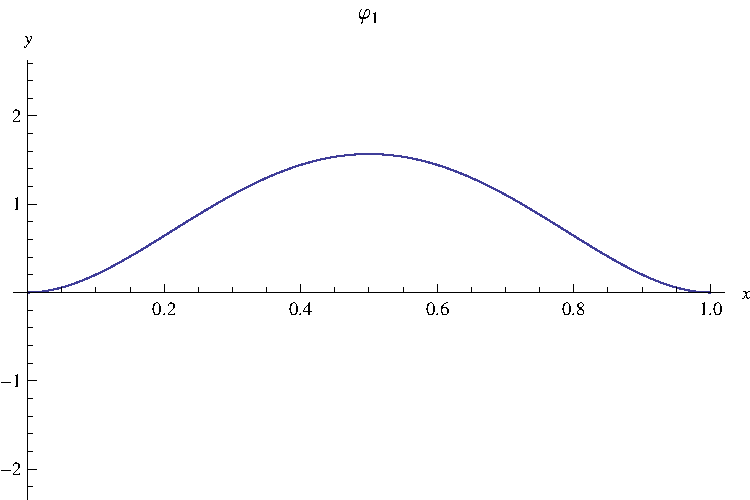
\includegraphics[width=6.7cm]{quintic_bspline_1.pdf}& 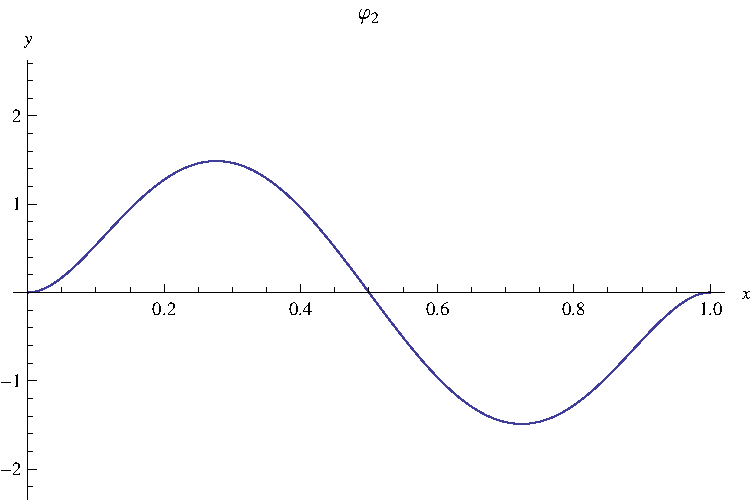
\includegraphics[width=6.7cm]{quintic_bspline_2.pdf}& 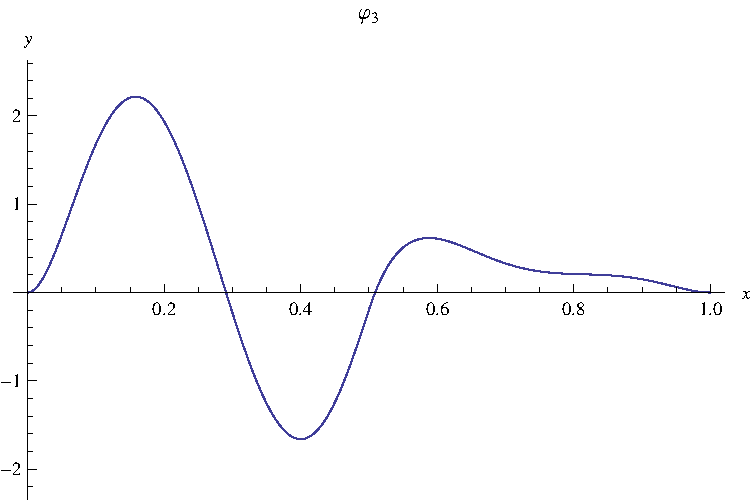
\includegraphics[width=6.7cm]{quintic_bspline_3.pdf} \\
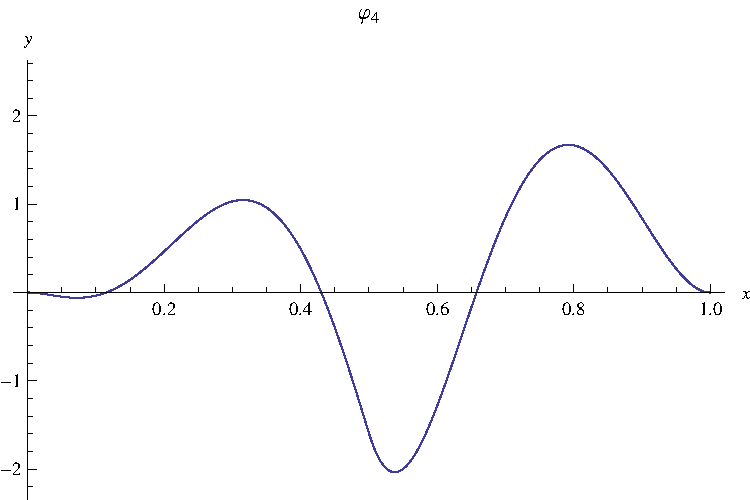
\includegraphics[width=6.7cm]{quintic_bspline_4.pdf}& 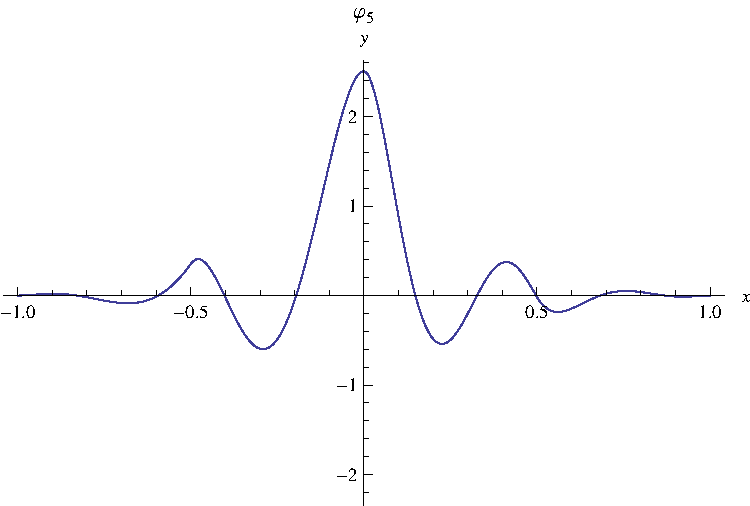
\includegraphics[width=6.7cm]{quintic_bspline_5.pdf}& 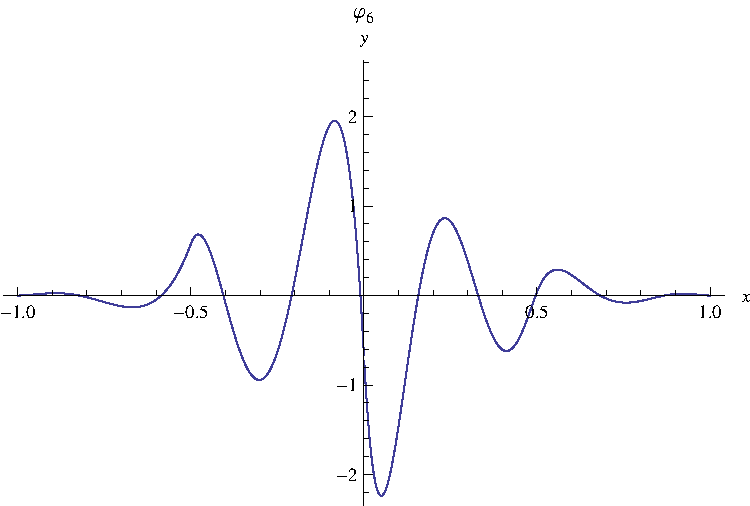
\includegraphics[width=6.7cm]{quintic_bspline_6.pdf} \\
\end{tabular} 
 \end{landscape}
 \begin{landscape}
 \subsection{Validation}$$ \begin{array}{l|llllll}
\int_{-1}^1 f_1(x)f_2(x) dx& \varphi_1(x)& \varphi_2(x)& \varphi_3(x)& \varphi_4(x)& \varphi_5(x)& \varphi_6(x) \\ \hline 
 \varphi_1(x) & 1.0000 & 0 & 0.\cdot 10^{(-786)} & 0.\cdot 10^{(-787)} & 0.\cdot 10^{(-720)} & 0.\cdot 10^{(-704)} \\ 
\varphi_2(x) & 0 & 1.0000 & 0.\cdot 10^{(-785)} & 0.\cdot 10^{(-786)} & 0.\cdot 10^{(-719)} & 0.\cdot 10^{(-703)} \\ 
\varphi_3(x) & 0.\cdot 10^{(-786)} & 0.\cdot 10^{(-785)} & 1.0000 & 0.\cdot 10^{(-784)} & 0.\cdot 10^{(-717)} & 0.\cdot 10^{(-702)} \\ 
\varphi_4(x) & 0.\cdot 10^{(-787)} & 0.\cdot 10^{(-786)} & 0.\cdot 10^{(-784)} & 1.0000 & 0.\cdot 10^{(-717)} & 0.\cdot 10^{(-702)} \\ 
\varphi_5(x) & 0.\cdot 10^{(-720)} & 0.\cdot 10^{(-719)} & 0.\cdot 10^{(-717)} & 0.\cdot 10^{(-717)} & 1.0000 & 0.\cdot 10^{(-702)} \\ 
\varphi_6(x) & 0.\cdot 10^{(-704)} & 0.\cdot 10^{(-703)} & 0.\cdot 10^{(-702)} & 0.\cdot 10^{(-702)} & 0.\cdot 10^{(-702)} & 1.0000 \\ 
\end{array} $$
$$ \begin{array}{l|llllll}
\int_{-1}^1 f_1(x)f_2(x-1) dx& \varphi_1(x-1)& \varphi_2(x-1)& \varphi_3(x-1)& \varphi_4(x-1)& \varphi_5(x-1)& \varphi_6(x-1) \\ \hline 
 \varphi_1(x) & 0 & 0 & 0 & 0 & 0.\cdot 10^{(-719)} & 0.\cdot 10^{(-703)} \\ 
\varphi_2(x) & 0 & 0 & 0 & 0 & 0.\cdot 10^{(-718)} & 0.\cdot 10^{(-702)} \\ 
\varphi_3(x) & 0 & 0 & 0 & 0 & 0.\cdot 10^{(-717)} & 0.\cdot 10^{(-701)} \\ 
\varphi_4(x) & 0 & 0 & 0 & 0 & 0.\cdot 10^{(-717)} & 0.\cdot 10^{(-701)} \\ 
\varphi_5(x) & 0 & 0 & 0 & 0 & 3.15978\cdot 10^{(-403)} & 3.74674\cdot 10^{(-403)} \\ 
\varphi_6(x) & 0 & 0 & 0 & 0 & -6.74792\cdot 10^{(-403)} & -7.80798\cdot 10^{(-403)} \\ 
\end{array} $$ 
\end{landscape} 
 \begin{landscape}
 \subsection{quintic BSpline dirichlet boundary Functions}
 \begin{eqnarray*}
 \varphi_{\text{left},1} & = & \begin{array}{cc}
 \{ & 
\begin{array}{cc}
 9012.876525410517719901663904183288254251285072148146181820688243073144830316566303804412305139684118 x^5-13917.37097095640098480996651628592416129950153621194770424225847560199791622165567535996759118403331 x^4+7623.274894793680692769441979796951364999040247076798920699155409859133968284975899095024588305641321 x^3-1721.298249932518381500538135313492838256776900375774960217603279293094929641683390175689637012063103 x^2+131.0763105407988782469072002590588693806104360174064670275936984567127635015097484151707170175522015 x & x\geq 0\land x<\frac{1}{2} \\
 -930.5001558408088801782838069699892277757115960918405657229967963610237767473510602113275613057223387 x^5+3766.140540706274607406002582514735564342015130074153708222805565002083905973266891672131125358212071 x^4-6008.720518437126754989072354418266120766148180484292640215680920926891730923978718171786688482057282 x^3+4714.776094099238387252371842103753748048539019621070586499817262803184565739068674955014482952605377 x^2-1815.452016508150538270117916161705252288136037626675256628830041028910678862513461026555595363275497 x+273.7560559805731787790996529314712884394416645075841678448849305115577148215076727825242368402376706 & x\geq \frac{1}{2}\land x<1
\end{array}

\end{array}\\ 
\varphi_{\text{right},1} & = & \begin{array}{cc}
 \{ & 
\begin{array}{cc}
 100.5020244968205796872236220401028899378764067106477510730774202923331194982072785810907374111249997 x^5-218.3783983423180613872919506062732925872634537207293458750192115352752297018201662776512223253081626 x^4+101.1475410264537755285917217743857767172271411646281964680517918014230856311230156119275091206662832 x^3-11.59962873183290393476402478323714811158761145553316418837264149189725713987210325545322963632394052 x^2 & x\geq 0\land x<\frac{1}{2} \\
 -1.270138713172610024099684552819618613664229974463390381298605381358277123845683344173597004915319794 x^5+1863.997685862241875982682708222010325284928365064643745484523492703344025982058713617956704625222272 x^4-5320.325753355411055943015243473868484566199128749074721450876595045447965910913823456728949104651772 x^3+5548.886105105341238227782866662576674274234565142654130226514342718804058684654682786391796271847793 x^2-2503.765004149932615459040463613476651436991934591499419950969538171829093565547046086511541209435810 x+412.4771052509331672156898167555777550576923631077396560721069031764872519335931564830655864219328362 & x\geq \frac{1}{2}\land x<1
\end{array}

\end{array}\end{eqnarray*}
\end{landscape}
\begin{landscape}
\subsection{BSpline Dirichlet boundary Graphics}
\begin{tabular}{c}
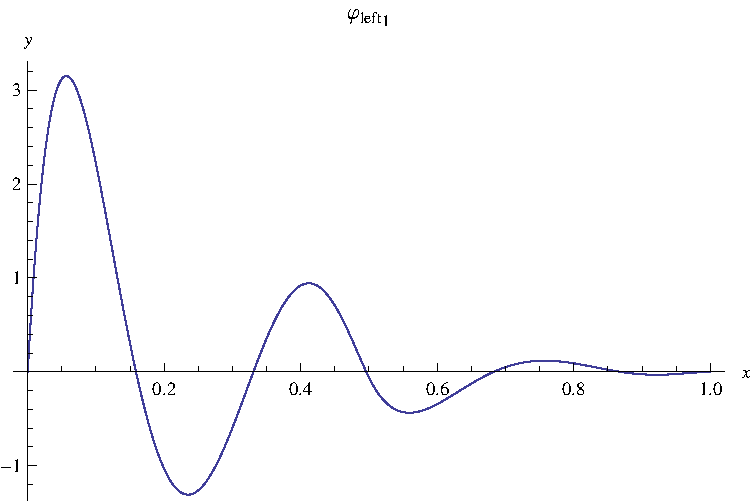
\includegraphics[width=20.cm]{quintic_bspline_dleft_1.pdf}\end{tabular} 
 \\ 
\begin{tabular}{c}
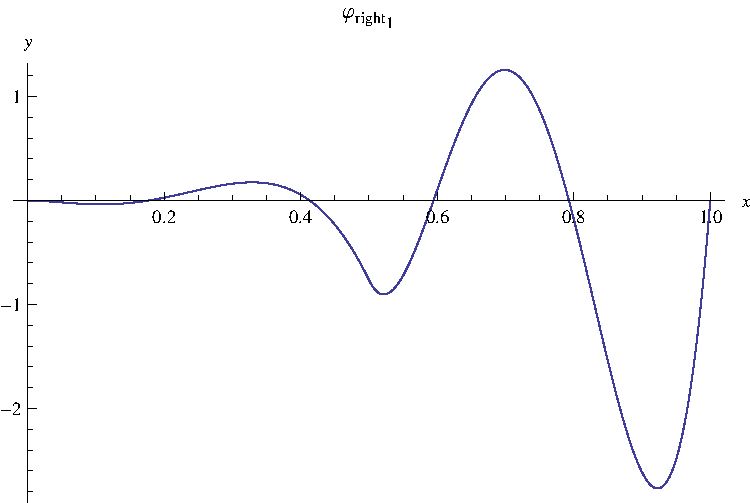
\includegraphics[width=20.cm]{quintic_bspline_dright_1.pdf}\end{tabular} 
 \end{landscape}
 \begin{landscape}
 \subsection{Validation}$$ \begin{array}{l|l}
\int_{-1}^1 f_1(x)f_2(x) dx& \varphi_{\text{left},1}(x) \\ \hline 
 \varphi_{\text{left},1}(x) & 1.0000 \\ 
\end{array} $$
$$ \begin{array}{l|llllll}
\int_{-1}^1 f_1(x)f_2(x) dx& \varphi_1(x)& \varphi_2(x)& \varphi_3(x)& \varphi_4(x)& \varphi_5(x)& \varphi_6(x) \\ \hline 
 \varphi_{\text{left},1}(x) & 0.\cdot 10^{(-696)} & 0.\cdot 10^{(-695)} & 0.\cdot 10^{(-693)} & 0.\cdot 10^{(-693)} & 0.56895 & -0.70307 \\ 
\end{array} $$ 
$$ \begin{array}{l|llllll}
\int_{-1}^1 f_1(x)f_2(x) dx& \varphi_1(x-1)& \varphi_2(x-1)& \varphi_3(x-1)& \varphi_4(x-1)& \varphi_5(x-1)& \varphi_6(x-1) \\ \hline 
 \varphi_{\text{left},1}(x) & 0 & 0 & 0 & 0 & 1.07049\cdot 10^{(-402)} & 1.23431\cdot 10^{(-402)} \\ 
\end{array} $$ 
$$ \begin{array}{l|l}
\int_{-1}^1 f_1(x)f_2(x) dx& \varphi_{\text{right},1}(x) \\ \hline 
 \varphi_{\text{right},1}(x) & 1.0000 \\ 
\end{array} $$
$$ \begin{array}{l|llllll}
\int_{-1}^1 f_1(x)f_2(x) dx& \varphi_1(x)& \varphi_2(x)& \varphi_3(x)& \varphi_4(x)& \varphi_5(x)& \varphi_6(x) \\ \hline 
 \varphi_{\text{right},1}(x) & 0.\cdot 10^{(-690)} & 0.\cdot 10^{(-689)} & 0.\cdot 10^{(-688)} & 0.\cdot 10^{(-688)} & -5.24022\cdot 10^{(-403)} & 1.09698\cdot 10^{(-402)} \\ 
\end{array} $$ 
$$ \begin{array}{l|llllll}
\int_{-1}^1 f_1(x)f_2(x) dx& \varphi_1(x-1)& \varphi_2(x-1)& \varphi_3(x-1)& \varphi_4(x-1)& \varphi_5(x-1)& \varphi_6(x-1) \\ \hline 
 \varphi_{\text{right},1}(x) & 0 & 0 & 0 & 0 & -0.66233 & -0.69923 \\ 
\end{array} $$ 
$$ \begin{array}{l|l}
\int_{-1}^1 f_1(x)f_2(x) dx& \varphi_{\text{left},1}(x) \\ \hline 
 \varphi_{\text{right},1}(x) & -1.73528\cdot 10^{(-402)} \\ 
\end{array} $$ 
\end{landscape} 
 \begin{landscape}
\section{Wavelets}
\subsection{Functions}
 \begin{eqnarray*}
\Psi_1 & = & \begin{array}{cc}
 \{ & 
\begin{array}{cc}
 -898.2660059315904809038479465200127239036759947215249794195298031805693822855531602769408819705656011 x^5-398.0733804916212919893552408567994536997196934982405798960401514992675346843589632163274635924579789 x^4+79.20843386197596531115642986854042721681402491456511896307205384146638544074285509016815813655332322 x^3+3.270202045230479103071790396647729604066411927523111198067336560605799133305737022677013333559697713 x^2 & x\geq 0\land x<\frac{1}{4} \\
 -1918.912461248592029592099480002557248900590930288648711833509323013904979280265026631996618195764793 x^5+34158.76681361618747202569318360160724911053700276501793575256054856984091786796285205458790687858873 x^4-47008.62610206318093599153460112077338995479072932860507381130711174508197520458688919420714352074360 x^3+24395.75109383924435132887118477673626331147535465604062381312065249463256066880450967531460091878049 x^2-5507.139481462367878371768242644867397305823628624822616991657570677110005552467206587683453038159220 x+454.0112972980835605021412336017952405678889070427092596647564152758829338283890468266597240753636648 & x\geq \frac{1}{4}\land x<\frac{1}{2} \\
 -19859.73917579184084692747227984276190166258868296036859824359850650831334523554815315076965039202438 x^5+57358.10606483588114235444883742936112356170020250864754177800692132733710935407874576781888487851254 x^4-63242.70271540864691939861887117419270581741909512038245329701076014635206178035116650194745470067576 x^3+32602.14935152238220882744953965803928319204606637674627672445376033532466270317346311832988239382205 x^2-7531.141556451487828062107221949918913526880368163597573798283258753595024037044921869392417566882439 x+554.3644786682879900447348399214444364367178743929068933496738270909679278522765551168626459995942795 & x\geq \frac{1}{2}\land x<\frac{3}{4} \\
 17370.67362174486205666597681958289655459905434541362910516713982076156011404251734486824093163472239 x^5-78806.54493181921727147792590223777392482048678152473282171296588464387303445235068277140275941417888 x^4+142637.0045637399908941218056936428954790855921973332918171882828901405204007156786400579901186108508 x^3-128732.9011413773292250770136138258377494394429133581290191202911466138288913114649818296408346140270 x^2+57927.60021008724457037042965775960198790878463374716834769189805757378814807271005022971769287860499 x-10395.83232237555102460327265492178234733350148161122742921406373721816673706709037055490514909597237 & x\geq \frac{3}{4}\land x<1
\end{array}

\end{array}\\
\Psi_2 & = & \begin{array}{cc}
 \{ & 
\begin{array}{cc}
 -286.0624274334967085241575483134198467429487137503161585601010009090159066619509206820332780083793634 x^5+1302.016252579095013875991258103787323104472359803290919547923124202786001549146060649572728422407064 x^4-360.6927077977122690858001304146604065997374365722956584711923357849783565502856800364679799908780784 x^3+21.49933690705123802247565322682257640707211966196365382350272670057584689023427109881158287420898671 x^2 & x\geq 0\land x<\frac{1}{4} \\
 -1996.050222120488094093689565363844867632926546198676419420487247782376267953888136766453223833364389 x^5-18932.46664662256612435454176240725208786092253509114640706065993213400758683571684303609049369148495 x^4+29270.42114006676255177065770865796383249907581642140347606954426410895664599776372296611429386124998 x^3-15557.05373101004196939322655413779528416727876110128895992050118661886417534833532222905780248633728 x^2+3531.496067799041696436078494846147962330742515916217088403579704084902116972062613832953294782011614 x-291.4897452970690138752371237649860746491612132241957850947824423040753963354657976420572718246811599 & x\geq \frac{1}{4}\land x<\frac{1}{2} \\
 -339972.0374752766916390032025050231544483147374376723647838236110366019395982505939441095915218448648 x^5+1.103110532758835382886875535355505084269751966213843192880011708432148276229150217922279392602175100\times 10^6 x^4-1.420936898794370638305227891066733978707454236429406232203612023788732840018629053145867771203104998\times 10^6 x^3+908035.9830868898952048232515437109554959014897212405392138101190049743669022720821848886979127370668 x^2-287810.0544853905057328623037867712798476164202529365263552260724460120098294534890595223991275214053 x+36191.00345744740506192119554900036535484689312489532990919315918708426600612320890450767107596315506 & x\geq \frac{1}{2}\land x<\frac{3}{4} \\
 54734.11503331595327440210855931185917896714919438436178843878799448152034146278423225598347829662478 x^5-248732.0194253080495587059396216353197341778838619254938370776574580138075869884479268642764549549302 x^4+450849.5971738188046605203540685928512891565265738433853073633575483299020136707234943119449891603525 x^3-407384.6723206224373343564987658067566632895335973584161135106786260060044036107587532352273314904243 x^2+183478.0556544408925499651510158169425009852769489668427110479744666699314068492175697118081238363881 x-32945.07611564516359182517525627957657164153525791067985626178392546154177138351861618023280484801087 & x\geq \frac{3}{4}\land x<1
\end{array}

\end{array}\\
\Psi_3 & = & \begin{array}{cc}
 \{ & 
\begin{array}{cc}
 -82015.95615489536134081622400003005089316159868911203877684829158449643880476618219344031198553326598 x^5+55250.12691644174314063121229155866322479043906241542457489353694902720353903006732030406694380251040 x^4-11507.73093007970435042920130059786449590324259273554951719450746706215559361947077081049938805449435 x^3+720.9076604179753460669317403809661972654904139694494145271366442202683757085165827660705492897804018 x^2 & x\geq 0\land x<\frac{1}{4} \\
 30383.91761410816517647805735075406410770884446871317183968925928036271906840743707583474264186664394 x^5-67930.40883361607596032313826314374568850756337119348166365676248031611205918367791355837621446270120 x^4+59286.86617511439107597503460955835449887216706493506977147763038525345242088232888883493214386705221 x^3-25158.20548443399809419961741112195446647296594827711546151066609717922249271246291643650655063960513 x^2+5169.043065029857394201223319633567581319213179484324316448020197395245729169339139181144424429574020 x-409.5733084267529000726549588129691031274827682718030929935198768243663230476128560249611569956778161 & x\geq \frac{1}{4}\land x<\frac{1}{2} \\
 421.7635208361636978820989070816734834412653513311497999574067461395145038601580396711152692664914485 x^5-1701.381063949689249460410887446048008988448107954140456204736110201341506386533972134186075777874950 x^4+2703.663116512400618956783774418338708513797860297383222127783328374808058107879416786279304372285516 x^3-2111.181841780922597834369669544589694733012882979021891991369399779003326638458615047835944343992432 x^2+808.0809856425818472295370302099878826720978602267069426312995245413759851986246699180019323501708714 x-120.9447172605343167736391547193623709057000809220776165203840890753537141416695391933744858670804545 & \left(x\geq \frac{1}{2}\land x<\frac{3}{4}\right)\lor \left(x\geq \frac{3}{4}\land x<1\right) \\
 619.6894049666466980866523970199883234031640059979575665865165120436301189904204279118548264302263825 x^5+2625.109556792380798062051163769475096146080537211332692679230442045066331703396366887981809571157698 x^4+4402.764281656523403551742816613515608072641250430843408334937607076083177938990284687106494215923476 x^3+3649.509012947861794142271863977746234582545326190915620263025730760642722879508766762301264337903816 x^2+1492.716383262443079444257948092904412515669019944843953305577848255150643803530007455936152161536085 x+240.5515001453705888783301339791870132628484129713966152847757945691548861500355864046143988986244292 & x\geq -1\land x<-\frac{1}{2} \\
 -31091.56027382485085504412243974064907683079399109903686441550587274791093952733617298425136802082622 x^5-63175.85340750475861880526717476245075754917649531311633995806934358416455831569739688164161980329925 x^4-48621.16465930064856839236336795209754294660439991654497301859225332299590564413820021893139325781244 x^3-17554.19895379773169054555944041893854548058065655467517627433608888801685235025775222447416141505102 x^2-2933.760835291498149365785750657834243557539367209619313847154473661458482961638091956089386907391352 x-178.1676022585112358288764798582373165367376140893638782554231069497783963254844277103611043725094040 & x\geq -\frac{1}{2}\land x<-\frac{1}{4} \\
 30848.20789296131370996932090193362410845136311821042472681816361517270829814920927874426450569414640 x^5+4920.822111473805818505945505551377647864055884822185863834188000891899461266217160378697383476077566 x^4-2051.813155509240001920395065688138182262177395929085314618462721058379005193330469416649787102623482 x^3-315.7327151501931807300637802593625524854115810746511087464455206534773622339279322108370093850034421 x^2 & x\geq -\frac{1}{4}\land x<0
\end{array}

\end{array}\\
\Psi_4 & = & \begin{array}{cc}
 \{ & 
\begin{array}{cc}
 -99353.80261103454217041473776586727214509509504738623634518565089276618931215752034669267431264869575 x^5+65780.40711195016934033310251321336121462867448489496516235248271883391082554297650918505964835415654 x^4-13234.21114885499125757368908310788990335635057198964494297314056134269495315365274308026510165692062 x^3+776.8134320364975365066824698892468158947136635654002965608841176528830464452459779545690820445512736 x^2 & x\geq 0\land x<\frac{1}{4} \\
 41547.27607763048111719173968169952831236003676789527250748281079886039473910902002751621308852633187 x^5-94588.64974872312833052611085472728821576761241903713033847079413349704934729531607320771494575318459 x^4+83781.25048422466201464425011294525298959522128067220323963045046948520231467178240282066237331249789 x^3-35965.68328695302001185236694431458084333091980945913488250472282845547062094997656076284901538210992 x^2+7451.941163946416153981297930690451055149494402366710054317404065630049387031435849218066227234073690 x-593.6029153615231418787985926370751845223878501703615431797748115487374101678453782235965083602274485 & x\geq \frac{1}{4}\land x<\frac{1}{2} \\
 805.2503962816907887077954281670549739200606258479405804229840280623739270571851123731661457480538348 x^5-3250.624079432285776161642794583599288211315464087722365542732518403359715099789869761522772220031723 x^4+5169.899796432865813039429246884369574685300033705517730925497413929012503726195708708861382821167807 x^3-4041.096136591227271812238888232572668296300969053043176804043395654726098024437827244497825895742486 x^2+1548.737220204546265613784073311158895781660564100719720887604482823983909983522445542671863467839271 x-232.1671968955898193871270655464114878794047905134124898893100107572845276426755696186787939212867032 & \left(x\geq \frac{1}{2}\land x<\frac{3}{4}\right)\lor \left(x\geq \frac{3}{4}\land x<1\right) \\
 -394.1410173904243938097672913216028604724659377697727058978946895793875770298562863839034424535524923 x^5-1679.083499621953693383649741484657141475834857162378305819536791736786147642870553677500507083616729 x^4-2832.363739471369657321739903320691734324848355404665619628325315580786210326971263089032986661970282 x^3-2361.525781394483631265364329944662920151016971139553813933888547376141301674770113187430995486797058 x^2-971.5892559105510950512714592578649008684986158657604627714748670601306777908272198982478470543877279 x-157.4847317559078215337645824708394340389610807382666685442695331073770158300141025062527735994967142 & x\geq -1\land x<-\frac{1}{2} \\
 20003.90586324015224385660992898478661181774882416933545388738021719316348790958964761162329584535568 x^5+40836.71617443708709498461492598935189425242194610240136921592693266478161210179556011186977423573834 x^4+31529.34499579041103236718211926280225635457496795647710589607504966449612201154447562491284156084651 x^3+11407.05108230276219830493602191145457985258343651955497928001799704565045133403097786094246531453758 x^2+1909.216243172824412165726828051889913898970587798909823883964857262060998042843269635749277521103045 x+116.1888791602065315473324724603944534548544957059825174740970966654754111722513901634202200051483004 & x\geq -\frac{1}{2}\land x<-\frac{1}{4} \\
 -19952.45091930999820483532537254664027915788055947476067096308821349021621708522115589348307914904490 x^5-4049.352781052259206061180869456208945992504361794749595415639531655358052664609409538451317799330598 x^4+902.8440565151365343809493166774157981278883690243747015307453052454366456775546432027594611760958789 x^3+153.6441763466884729573408165527785723215150520107432955770640133308290899925390756255083113592148481 x^2 & x\geq -\frac{1}{4}\land x<0
\end{array}

\end{array}\\
\Psi_5 & = & \begin{array}{cc}
 \{ & 
\begin{array}{cc}
 153451.7364999095432788057480236068071424464011322057445925787544220199302449225585765781825968307653 x^5-110882.2935652959225873664564632912339542609434827015239798343671463248358048615122199681780580894641 x^4+26264.45855175797776147540840454120861104824344031153596667056363964868426349291827368620823979285453 x^3-2024.667891664886812894765721313122777493271882170098120007746972577765738637661655029685199763867929 x^2-9.693813073423225862781595865868172740412156135638093350409351220188403465105781784922845157873781800 x+2.438116519659855111148348515109960845686426834850900874182875238691279904678831078511042843137322063 & x\geq 0\land x<\frac{1}{4} \\
 -28981.31656051229331052447704246905605934783133051936834050710153410508334778748651806055070911984964 x^5+56965.86951866082625552638696994499232038204375037469748052963317861677251914154292891219376142971063 x^4-44078.19023925018630639501919495522755517632560549463135841644275274354545793535659529544574524111064 x^3+16800.87136131544545168185946212160244196171275450270143116901079955484664707045884722408753501671388 x^2-3160.581416410491402220835768933118940305940877663045474783391434878735372068937373528109569192396686 x+235.1680927347708458518158773143948428910689700255501417575352902140185134171899616887044570182330122 & x\geq \frac{1}{4}\land x<\frac{1}{2} \\
 -7358.942985420237559944127492233853183637909998362049812750001479582817216360838350879280640560136645 x^5-12517.96593660429733348375113190588795830146323950696697236194491350799492893082483540453933968094635 x^4-8159.079276904341652552817047349815636072297826158000516185215662939718889848567099895690573940341008 x^3-2494.340710721150260122111893160393965941382287887120474660404368354372275487971948722943639958646329 x^2-338.3472563540560229424698980150940663848312871415838438655087888273983572310245071494239016728723674 x-13.34613191505647898798751112113080148017067420886974744748540410328904929699968357878270807647063176 & x\geq -\frac{1}{2}\land x<-\frac{1}{4} \\
 5660.845841254593672479166442378482838317182116697511426318279721760394929150515444840981295198192422 x^5-14732.49297265374417144920420182835076667834004725047648516678853052087251176825391882909924953371587 x^4-8469.481907084161939029288394102063323776318839104533981844888950756132836110810748607102855291253188 x^3-1168.033429929150823629195490832932834636821519017726223250872789517028675515759973187328411838085305 x^2-9.693813073423225862781595865868172740412156135638093350409351220188403465105781784922845157873781800 x+2.438116519659855111148348515109960845686426834850900874182875238691279904678831078511042843137322063 & x\geq -\frac{1}{4}\land x<0 \\
 485.8480651417671349815561183878587238318298070864305130821375446972997476487276479157874077160064397 x^5-1967.151399713128918842395713550452210686668784460579464502607132970847529600769640110278950095317575 x^4+3139.864580763259992003370077464869789712298382350672016976742425670008375353331030943104835159436507 x^3-2464.998812711052999174295687985441034329385092513355513940699893147144952982897883627831468452287328 x^2+949.7691562760060228002834058387879231094011403848602695509133176811561600652429952885271932275032382 x-143.3315897568512317685182001556231916374754528480278211664862619304718004836341504093090175553412812 & x\geq \frac{1}{2}\land x<1 \\
 105.7512487891269703149105970788810086480771790974790310759408582103643939208838525749638824680636599 x^5+380.3201663483526959742717933051347273301962004474643572887615060563275470849294239852584340393683056 x^4+521.3387394747794858720810413112967600365165568690734370837743665736702910113544535971426351058660705 x^3+333.5978423452145076777394244525039242305497048011021044488806531612466717056101452945558864154066715 x^2+95.70388771386649006176991279725143443194864529744617142177993977497068911245536286389819133037005442 x+8.875867284205742596750333429790551555796476015432177843853005341431155254154099756190388449524807751 & x\geq -1\land x<-\frac{1}{2}
\end{array}

\end{array}\\
\Psi_6 & = & \begin{array}{cc}
 \{ & 
\begin{array}{cc}
 -277851.9773872128179647305909938375374825734957208221595332119901478885277214096718225073337784845228 x^5+211459.0648308560730149391779171856313986457348180352685611141057787110819543840563139315160790451360 x^4-56233.48215408527383906250028068341321783667290904640201557466899142124075616128884491853912177096082 x^3+5957.798475990192174410021575119406569868470278451211246191310496823080468076902250578200250696508836 x^2-191.1708035545858561621724532939383212034256490958622338482839134984607825144819144491238921682142309 x-0.8789777869131265925491521883024282860826612909220105922154853029864390868541361439299542950515661974 & x\geq 0\land x<\frac{1}{4} \\
 33612.47353307001958897946992101426370729245985254364554719673591460702073756155155100030359944704529 x^5-66904.89093008658569203552154810976290746907054092052022324731947873647848660781261812635126645397123 x^4+52471.58263010045499829975259069078768543594910577570789849454419312282226523001016098818310876314752 x^3-20258.60243539538847027559719997340229282937986254059290289143906048070098375980689307401379893457611 x^2+3849.287183125522307390233610207566342924488683763330150350969540733774473615714195509268380978151193 x-287.7903554088998382460097573114497576042978434815218088166132866715611731581874864323971871403259651 & x\geq \frac{1}{4}\land x<\frac{1}{2} \\
 -2431.179498243084838622219791270613610096681272809073607914490421053601748761917969954608772660180457 x^5-2271.843784071766638920098938417531242633416593201347711734699982771800911393625746280415690300541919 x^4+285.7987940738320447963329770253396668659914198106639756480620963229711465552764079144987362158594408 x^3+944.7655773705986579520650502931913013048880827083242950419208292272566315924364488471131558953012506 x^2+350.5006613483442960859507100426203436012155462975554933422511689709283051604916221040244124100812668 x+40.59605880653609883725236180221173656953314112356927774829313643212784106346501624892322894029363214 & x\geq -\frac{1}{2}\land x<-\frac{1}{4} \\
 -1371.123749827107225657705432839078241383980957607503060460899398031553857076168361320555970099899182 x^5-35071.82800265226187159934923642289084421314757560920447050953118346529838682087644883981384857717314 x^4-19670.89252252979295492951543678237855091294179773335760885035955825600911440815207354925066253105149 x^3-3480.930141166559991850041802180918559433688035793975809169297656755153211421415372900897020406791452 x^2-191.1708035545858561621724532939383212034256490958622338482839134984607825144819144491238921682142309 x-0.8789777869131265925491521883024282860826612909220105922154853029864390868541361439299542950515661974 & x\geq -\frac{1}{4}\land x<0 \\
 -259.1389925324026778081508174267469539577273172263270114215123651564668061258679121882503614881794741 x^5+1048.953318429717843874508740710079320853068749735818510147265958911307939349133593919229663468675959 x^4-1673.760677312023423578518745306450133977875717956847044428741978902570482985216703262101182346852737 x^3+1313.514702597114440338819111627780756174897456811801637281818948970499026747282368204036252399742326 x^2-505.8656843150165963993628630427936240398061725647011247589139710961843313061094413574358041927329058 x+76.29733313261041357270457343813063494744300120025503318008340727341465432077809468452143215934683200 & x\geq \frac{1}{2}\land x<1 \\
 16.61315369308616720386770849055348461690917970967625330997678139485924762273866955325110386303003375 x^5+35.01414863544817466249343139776460287395677591673334296698226850388860474337204168684494633252080296 x^4-2.175610859074556262831634641144555701391168411991112238410283503278300805760779388867569675386042568 x^3-53.30800835260597502022712733014924063790063745137173209989626806503362748995039927586688220484895964 x^2-43.09835805162641862132416759857382576034656454821802216651651857897417170282364140400678936860674850 x-10.36695550045700732255439781678025908088469171589449196203602112624820213926739365060131930863460063 & x\geq -1\land x<-\frac{1}{2}
\end{array}

\end{array}\end{eqnarray*}
\end{landscape}
\begin{landscape}
\subsection{Graphics}
\begin{tabular}{ccc}
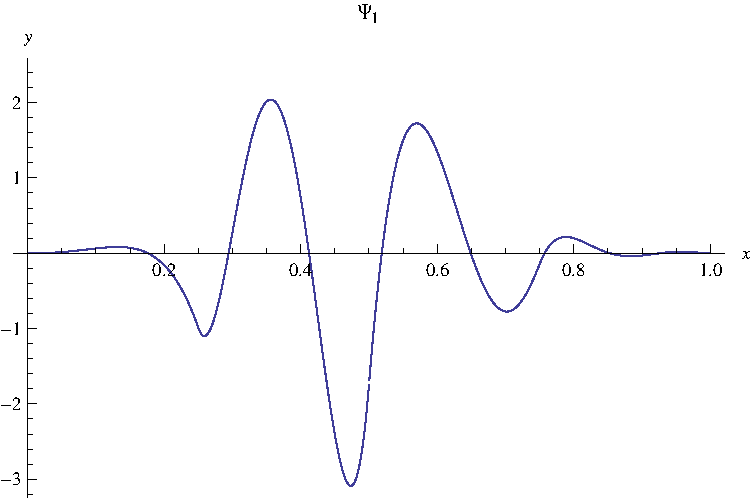
\includegraphics[width=6.7cm]{quintic_wavelet_1.pdf}& 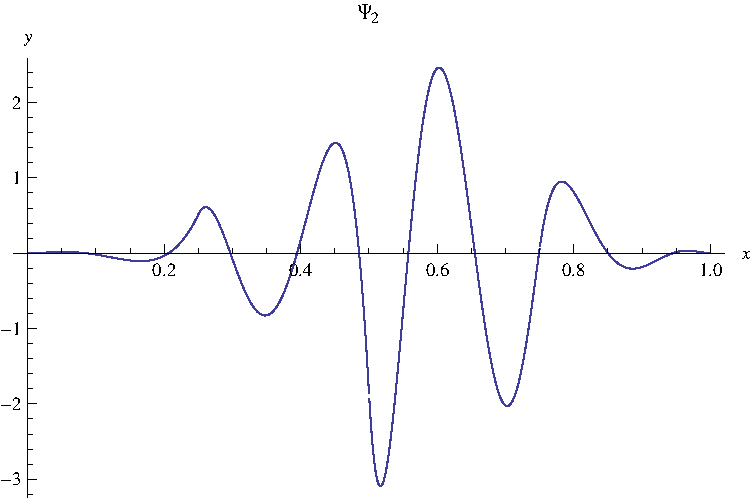
\includegraphics[width=6.7cm]{quintic_wavelet_2.pdf}& 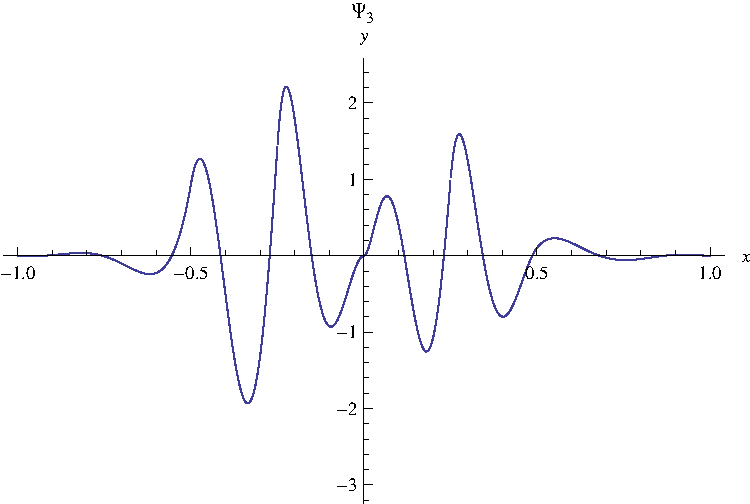
\includegraphics[width=6.7cm]{quintic_wavelet_3.pdf} \\
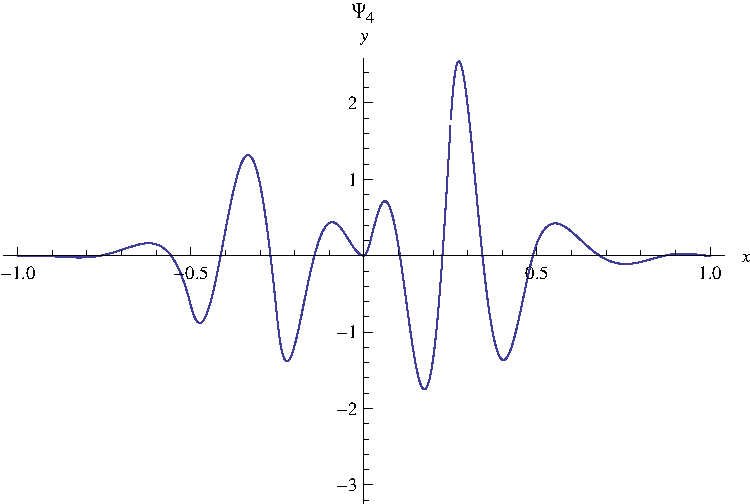
\includegraphics[width=6.7cm]{quintic_wavelet_4.pdf}& 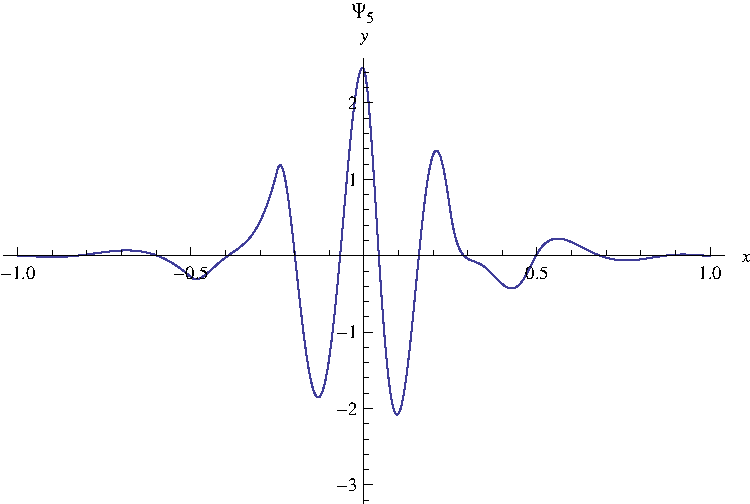
\includegraphics[width=6.7cm]{quintic_wavelet_5.pdf}& 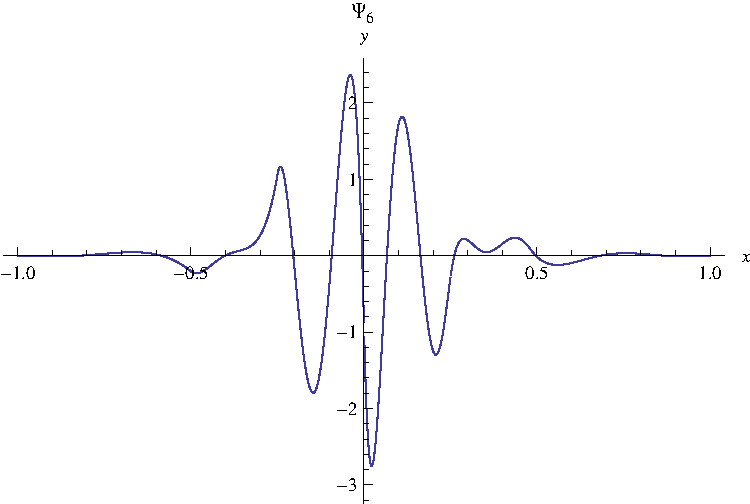
\includegraphics[width=6.7cm]{quintic_wavelet_6.pdf} \\
\end{tabular} 
 \end{landscape}
 \begin{landscape}
 \subsection{Validation}$$ \begin{array}{l|llllll}
\int_{-1}^1 f_1(x)f_2(x) dx& \Psi_1(x)& \Psi_2(x)& \Psi_3(x)& \Psi_4(x)& \Psi_5(x)& \Psi_6(x) \\ \hline 
 \Psi_1(x) & 1.0000 & 0.\cdot 10^{(-375)} & 0.\cdot 10^{(-399)} & 0.\cdot 10^{(-399)} & 0.\cdot 10^{(-399)} & 0.\cdot 10^{(-400)} \\ 
\Psi_2(x) & 0.\cdot 10^{(-375)} & 1.0000 & 0.\cdot 10^{(-377)} & 0.\cdot 10^{(-377)} & 0.\cdot 10^{(-377)} & 0.\cdot 10^{(-377)} \\ 
\Psi_3(x) & 0.\cdot 10^{(-399)} & 0.\cdot 10^{(-377)} & 1.0000 & 0.\cdot 10^{(-479)} & 1.5428\cdot 10^{(-403)} & -5.00113\cdot 10^{(-403)} \\ 
\Psi_4(x) & 0.\cdot 10^{(-399)} & 0.\cdot 10^{(-377)} & 0.\cdot 10^{(-479)} & 1.0000 & -1.08539\cdot 10^{(-403)} & 3.5096\cdot 10^{(-403)} \\ 
\Psi_5(x) & 0.\cdot 10^{(-399)} & 0.\cdot 10^{(-377)} & 1.5428\cdot 10^{(-403)} & -1.08539\cdot 10^{(-403)} & 1.0000 & 0.\cdot 10^{(-650)} \\ 
\Psi_6(x) & 0.\cdot 10^{(-400)} & 0.\cdot 10^{(-377)} & -5.00113\cdot 10^{(-403)} & 3.5096\cdot 10^{(-403)} & 0.\cdot 10^{(-650)} & 1.0000 \\ 
\end{array} $$
$$ \begin{array}{l|llllll}
\int_{-1}^1 f_1(x)f_2(x-1) dx& \Psi_1(x-1)& \Psi_2(x-1)& \Psi_3(x-1)& \Psi_4(x-1)& \Psi_5(x-1)& \Psi_6(x-1) \\ \hline 
 \Psi_1(x) & 0 & 0 & 0.\cdot 10^{(-397)} & 0.\cdot 10^{(-398)} & 0.\cdot 10^{(-398)} & 0.\cdot 10^{(-398)} \\ 
\Psi_2(x) & 0 & 0 & 0.\cdot 10^{(-375)} & 0.\cdot 10^{(-375)} & 0.\cdot 10^{(-375)} & 0.\cdot 10^{(-375)} \\ 
\Psi_3(x) & 0 & 0 & 2.48874\cdot 10^{(-402)} & -1.46639\cdot 10^{(-402)} & 1.27977\cdot 10^{(-402)} & 5.31435\cdot 10^{(-403)} \\ 
\Psi_4(x) & 0 & 0 & 3.29275\cdot 10^{(-402)} & -1.82204\cdot 10^{(-402)} & 2.55022\cdot 10^{(-402)} & 1.16037\cdot 10^{(-402)} \\ 
\Psi_5(x) & 0 & 0 & 4.12086\cdot 10^{(-403)} & -2.24184\cdot 10^{(-403)} & 3.60988\cdot 10^{(-403)} & 1.79973\cdot 10^{(-403)} \\ 
\Psi_6(x) & 0 & 0 & -3.41281\cdot 10^{(-403)} & 1.96339\cdot 10^{(-403)} & -2.17018\cdot 10^{(-403)} & -1.01341\cdot 10^{(-403)} \\ 
\end{array} $$ 
$$ \begin{array}{l|llllll}
\int_{-1}^1 f_1(x)f_2(x) dx& \varphi_1(x)& \varphi_2(x)& \varphi_3(x)& \varphi_4(x)& \varphi_5(x)& \varphi_6(x) \\ \hline 
 \Psi_1(x) & 0.\cdot 10^{(-401)} & 0.\cdot 10^{(-400)} & 0.\cdot 10^{(-399)} & 0.\cdot 10^{(-399)} & 0.\cdot 10^{(-400)} & 0.\cdot 10^{(-399)} \\ 
\Psi_2(x) & 0.\cdot 10^{(-379)} & 0.\cdot 10^{(-378)} & 0.\cdot 10^{(-377)} & 0.\cdot 10^{(-377)} & 0.\cdot 10^{(-377)} & 0.\cdot 10^{(-377)} \\ 
\Psi_3(x) & 1.7845\cdot 10^{(-402)} & 2.94864\cdot 10^{(-403)} & -8.89113\cdot 10^{(-403)} & -1.0968\cdot 10^{(-402)} & 1.81245\cdot 10^{(-403)} & -2.13337\cdot 10^{(-403)} \\ 
\Psi_4(x) & -1.16132\cdot 10^{(-402)} & -1.91876\cdot 10^{(-403)} & 5.78582\cdot 10^{(-403)} & 7.13815\cdot 10^{(-403)} & -1.27464\cdot 10^{(-403)} & 1.49748\cdot 10^{(-403)} \\ 
\Psi_5(x) & 1.99657\cdot 10^{(-403)} & 3.32746\cdot 10^{(-404)} & -1.00121\cdot 10^{(-403)} & -1.22023\cdot 10^{(-403)} & 0.\cdot 10^{(-666)} & 0.\cdot 10^{(-666)} \\ 
\Psi_6(x) & -3.29994\cdot 10^{(-403)} & -5.39434\cdot 10^{(-404)} & 1.63096\cdot 10^{(-403)} & 2.04243\cdot 10^{(-403)} & 0.\cdot 10^{(-651)} & 0.\cdot 10^{(-651)} \\ 
\end{array} $$ 
$$ \begin{array}{l|llllll}
\int_{-1}^1 f_1(x)f_2(x-1) dx& \varphi_1(x-1)& \varphi_2(x-1)& \varphi_3(x-1)& \varphi_4(x-1)& \varphi_5(x-1)& \varphi_6(x-1) \\ \hline 
 \Psi_1(x) & 0 & 0 & 0 & 0 & 0.\cdot 10^{(-400)} & 0.\cdot 10^{(-399)} \\ 
\Psi_2(x) & 0 & 0 & 0 & 0 & 0.\cdot 10^{(-377)} & 0.\cdot 10^{(-377)} \\ 
\Psi_3(x) & 0 & 0 & 0 & 0 & -1.43007\cdot 10^{(-402)} & -1.49099\cdot 10^{(-402)} \\ 
\Psi_4(x) & 0 & 0 & 0 & 0 & -2.89206\cdot 10^{(-402)} & -3.25118\cdot 10^{(-402)} \\ 
\Psi_5(x) & 0 & 0 & 0 & 0 & -3.81446\cdot 10^{(-403)} & -4.4271\cdot 10^{(-403)} \\ 
\Psi_6(x) & 0 & 0 & 0 & 0 & 2.29686\cdot 10^{(-403)} & 2.52918\cdot 10^{(-403)} \\ 
\end{array} $$ 
$$ \begin{array}{l|llllll}
\int_{-1}^1 f_1(x)f_2(x+1) dx& \varphi_1(x+1)& \varphi_2(x+1)& \varphi_3(x+1)& \varphi_4(x+1)& \varphi_5(x+1)& \varphi_6(x+1) \\ \hline 
 \Psi_1(x) & 0 & 0 & 0 & 0 & 0 & 0 \\ 
\Psi_2(x) & 0 & 0 & 0 & 0 & 0 & 0 \\ 
\Psi_3(x) & 5.85302\cdot 10^{(-403)} & -1.28218\cdot 10^{(-403)} & 2.17745\cdot 10^{(-403)} & -9.07362\cdot 10^{(-403)} & -2.82407\cdot 10^{(-403)} & 6.96029\cdot 10^{(-403)} \\ 
\Psi_4(x) & -3.73128\cdot 10^{(-403)} & 8.17885\cdot 10^{(-404)} & -1.38925\cdot 10^{(-403)} & 5.78562\cdot 10^{(-403)} & 1.46978\cdot 10^{(-403)} & -3.75896\cdot 10^{(-403)} \\ 
\Psi_5(x) & 1.99657\cdot 10^{(-403)} & -4.28717\cdot 10^{(-404)} & 7.23162\cdot 10^{(-404)} & -3.0741\cdot 10^{(-403)} & -2.97642\cdot 10^{(-403)} & 6.22103\cdot 10^{(-403)} \\ 
\Psi_6(x) & 1.67481\cdot 10^{(-403)} & -3.49098\cdot 10^{(-404)} & 5.82778\cdot 10^{(-404)} & -2.55306\cdot 10^{(-403)} & -1.51877\cdot 10^{(-403)} & 3.03767\cdot 10^{(-403)} \\ 
\end{array} $$ 
\end{landscape} 
 \begin{landscape}
 \subsection{quintic Wavelet dirichlet boundary Functions}
 \begin{eqnarray*}
 \Psi_{\text{left},1} & = & \begin{array}{cc}
 \{ & 
\begin{array}{cc}
 149707.1332023004921139452568793055057389959576623004863613581346233088353091224176944300298391862307 x^5-101287.0159428906166854684529165578518730036364923837340167236336516600310666392825315510632662416054 x^4+21359.43378658060530580600487493038704695372702418890650717138941164475364515640273825465017384376112 x^3-1407.293118979408401367052702688564262946595417932397513146833389011684386344494097974501119510071143 x^2+7.295103312529101710495342668065336707789562345738685247467139970570627544947493232549926522927012636 x & x\geq 0\land x<\frac{1}{4} \\
 -54773.58224700003744692422178525585373267408187766172298859481673270394193962734095253384814131838959 x^5+122806.1545829473055903480296944920465526638630258512050593359519391230922531977322043557850887871738 x^4-107431.9018315128203050504899221639834622950758422876008219761504435895988393874806692259973236319740 x^3+45672.64917640101151597664757728293015927316916492993525518992309544725471156387788177204577559262570 x^2-9396.359800230882729178560180885892003341105451745879365593202897654278482407430055158766895634288901 x+745.1062027716896525672938096538175097142901148778432560095062122101749937536881639720946774469491621 & x\geq \frac{1}{4}\land x<\frac{1}{2} \\
 -819.0702979056753096370064796619770822700114382797636933116046151199125477997403737290611024340856180 x^5+3304.801824294092265656399034055451624290698003201395493997729312727506308981920702893299457083667849 x^4-5252.990548112360234134999093557690945962231922753527656812237696964141805108435343909984335079816373 x^3+4103.118527834685959909403720598621972456219674302275942386925751305295677787380686321044684330579270 x^2-1571.121218980283731854373898436092192838478401750732423770032587028628437178436283840028679585952725 x+235.2617128695410500605767170016866243238040852803523375092198350798808033173106122647299756856075977 & \left(x\geq \frac{1}{2}\land x<\frac{3}{4}\right)\lor \left(x\geq \frac{3}{4}\land x<1\right)
\end{array}

\end{array}\\
\Psi_{\text{left},2} & = & \begin{array}{cc}
 \{ & 
\begin{array}{cc}
 -429577.3368217875197837817222973790577855461627110148474235587576490728223670652997579714446461523084 x^5+329339.3479489843229514792909652482379219684679716311566629140538382093391493400989969663977044028077 x^4-88891.49705366030938552227452953157975047316231150236983465727087231543528756510330883607463613013493 x^3+9731.393632624738664012120482973314427476592853225980775118409143184745171010353383103755079636606490 x^2-346.7185829495949136226308088381060022230438921873980499773421157422014117420242357510442296613726821 x & x\geq 0\land x<\frac{1}{4} \\
 47281.89365240012247123561507097829600452444165294951467087302163943081563392595501293755757868778509 x^5-93799.61532197898104339705955172365271221323829255016446945145954707283835483052676280620367771430705 x^4+73312.28987026031341086815164641034502319885420484775382900974716930073367806816329489831135445149078 x^3-28208.35829878889307002457933824539037802353030045658767664885284590605648424910893376490420699405772 x^2+5342.475693758333290958978730617149103887554737865891612584696893351717149135273099724559177098316197 x-398.2945111326382621213886793536023312933607529558582313343937826557280049633042451110635257146440326 & x\geq \frac{1}{4}\land x<\frac{1}{2} \\
 -369.0074201973113074120586728783890494898815868397953514110137534676109789314674362853903120817856313 x^5+1493.316779807094046764399818864277905904327378018239211464914497094568406601667642124680945523268915 x^4-2382.110639555261136493064944664282774105191567031701716584029904075355569511869904220916982488354635 x^3+1868.743588799182117279908727588703601984921179752271924310749600511065440413239947375173598725070996 x^2-719.3852771744004750779285322497252578221692362834187876739987098362829040402035691593684716692255903 x+108.4429683206967549387436033394155735279938323844047198933782697736156054686333201658212219910259457 & \left(x\geq \frac{1}{2}\land x<\frac{3}{4}\right)\lor \left(x\geq \frac{3}{4}\land x<1\right)
\end{array}

\end{array}\\ 
\Psi_{\text{right},1} & = & \begin{array}{cc}
 \{ & 
\begin{array}{cc}
 -744.832015341693105693155847660147897 x^5+572.199116796017880973833044074813140 x^4-121.223436994302465278711324223302533 x^3+6.28375850006296911565888524202639313 x^2 & x\geq 0\land x<\frac{1}{2} \\
 37253.7687773774143814332658620297112 x^5-110614.825126184333775892696598414683 x^4+128130.148235323273067415772521180281 x^3-72223.3873553102545379454821546825673 x^2+19760.0917333375905962465361928385733 x-2092.31680684211299336333589288580073 & x\geq \frac{1}{2}\land x<\frac{3}{4} \\
 -36962.1265413531678813751737760280763 x^5+178871.583048783480958314390708973816 x^4-343455.676455829632121309254147544387 x^3+327119.553814211227222069530409981036 x^2-154549.689008921800431318295710755938 x+28976.3551431098922536188025153735491 & x\geq \frac{3}{4}\land x<1
\end{array}

\end{array}\end{eqnarray*}
\end{landscape}
\begin{landscape}
\subsection{Wavelet Dirichlet boundary Graphics}
\begin{tabular}{cc}
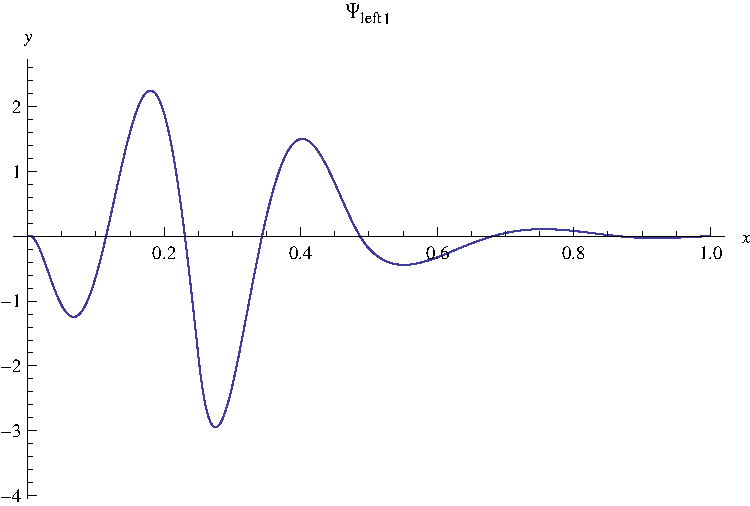
\includegraphics[width=10.cm]{quintic_wavelet_dleft_1.pdf}& 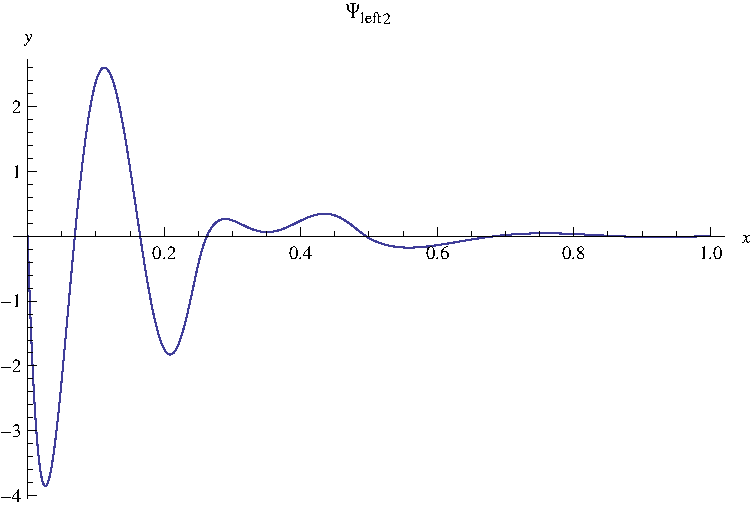
\includegraphics[width=10.cm]{quintic_wavelet_dleft_2.pdf} \\
\end{tabular} 
 \\ 
\begin{tabular}{c}
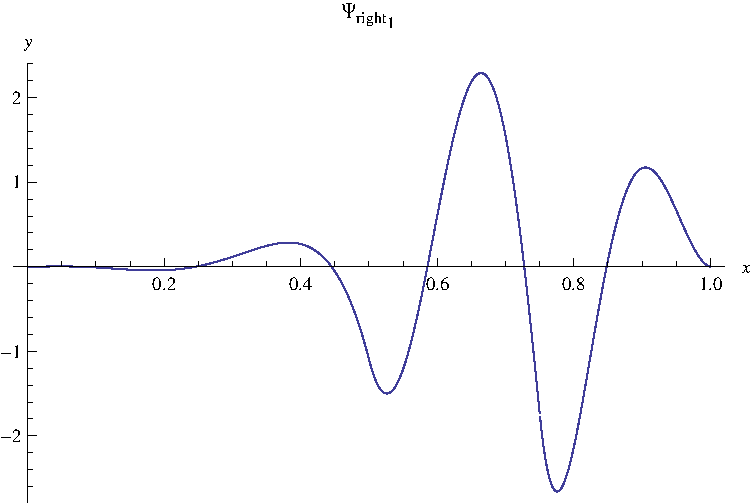
\includegraphics[width=20.cm]{quintic_wavelet_dright_1.pdf}\end{tabular} 
 \end{landscape}
 \begin{landscape}
 \subsection{Validation}$$ \begin{array}{l|ll}
\int_{-1}^1 f_1(x)f_2(x) dx& \Psi_{\text{left},1}(x)& \Psi_{\text{left},2}(x) \\ \hline 
 \Psi_{\text{left},1}(x) & 1.0000 & 0.\cdot 10^{(-205)} \\ 
\Psi_{\text{left},2}(x) & 0.\cdot 10^{(-205)} & 1.0000 \\ 
\end{array} $$
$$ \begin{array}{l|llllll}
\int_{-1}^1 f_1(x)f_2(x) dx& \varphi_1(x)& \varphi_2(x)& \varphi_3(x)& \varphi_4(x)& \varphi_5(x)& \varphi_6(x) \\ \hline 
 \Psi_{\text{left},1}(x) & 0.\cdot 10^{(-240)} & 0.\cdot 10^{(-239)} & 0.\cdot 10^{(-237)} & 0.\cdot 10^{(-237)} & -0.061420 & 0.016313 \\ 
\Psi_{\text{left},2}(x) & 0.\cdot 10^{(-208)} & 0.\cdot 10^{(-207)} & 0.\cdot 10^{(-205)} & 0.\cdot 10^{(-205)} & -0.21638 & 0.057472 \\ 
\end{array} $$ 
$$ \begin{array}{l|llllll}
\int_{-1}^1 f_1(x)f_2(x) dx& \varphi_1(x-1)& \varphi_2(x-1)& \varphi_3(x-1)& \varphi_4(x-1)& \varphi_5(x-1)& \varphi_6(x-1) \\ \hline 
 \Psi_{\text{left},1}(x) & 0 & 0 & 0 & 0 & 0.\cdot 10^{(-238)} & 0.\cdot 10^{(-238)} \\ 
\Psi_{\text{left},2}(x) & 0 & 0 & 0 & 0 & 0.\cdot 10^{(-206)} & 0.\cdot 10^{(-205)} \\ 
\end{array} $$ 
$$ \begin{array}{l|llllll}
\int_{-1}^1 f_1(x)f_2(x) dx& \Psi_1(x)& \Psi_2(x)& \Psi_3(x)& \Psi_4(x)& \Psi_5(x)& \Psi_6(x) \\ \hline 
 \Psi_{\text{left},1}(x) & 0.\cdot 10^{(-236)} & 0.\cdot 10^{(-236)} & -0.54968 & -0.82867 & 0.080129 & -0.025046 \\ 
\Psi_{\text{left},2}(x) & 0.\cdot 10^{(-204)} & 0.\cdot 10^{(-203)} & 0.\cdot 10^{(-205)} & -0.059861 & -0.53319 & 0.70911 \\ 
\end{array} $$ 
$$ \begin{array}{l|llllll}
\int_{-1}^1 f_1(x)f_2(x) dx& \Psi_1(x-1)& \Psi_2(x-1)& \Psi_3(x-1)& \Psi_4(x-1)& \Psi_5(x-1)& \Psi_6(x-1) \\ \hline 
 \Psi_{\text{left},1}(x) & 0 & 0 & 0.\cdot 10^{(-236)} & 0.\cdot 10^{(-236)} & 0.\cdot 10^{(-236)} & 0.\cdot 10^{(-236)} \\ 
\Psi_{\text{left},2}(x) & 0 & 0 & 0.\cdot 10^{(-204)} & 0.\cdot 10^{(-204)} & 0.\cdot 10^{(-204)} & 0.\cdot 10^{(-204)} \\ 
\end{array} $$ 
$$ \begin{array}{l|l}
\int_{-1}^1 f_1(x)f_2(x) dx& \varphi_{\text{left},1}(x) \\ \hline 
 \Psi_{\text{left},1}(x) & 0.\cdot 10^{(-237)} \\ 
\Psi_{\text{left},2}(x) & 0.\cdot 10^{(-205)} \\ 
\end{array} $$ 
$$ \begin{array}{l|l}
\int_{-1}^1 f_1(x)f_2(x) dx& \varphi_{\text{right},1}(x) \\ \hline 
 \Psi_{\text{left},1}(x) & 0.\cdot 10^{(-238)} \\ 
\Psi_{\text{left},2}(x) & 0.\cdot 10^{(-205)} \\ 
\end{array} $$ 
$$ \begin{array}{l|l}
\int_{-1}^1 f_1(x)f_2(x) dx& \Psi_{\text{right},1}(x) \\ \hline 
 \Psi_{\text{right},1}(x) & 1.0000 \\ 
\end{array} $$
$$ \begin{array}{l|llllll}
\int_{-1}^1 f_1(x)f_2(x) dx& \varphi_1(x)& \varphi_2(x)& \varphi_3(x)& \varphi_4(x)& \varphi_5(x)& \varphi_6(x) \\ \hline 
 \Psi_{\text{right},1}(x) & 0.\cdot 10^{(-29)} & 0.\cdot 10^{(-28)} & 0.\cdot 10^{(-27)} & 0.\cdot 10^{(-27)} & 0.\cdot 10^{(-27)} & 0.\cdot 10^{(-27)} \\ 
\end{array} $$ 
$$ \begin{array}{l|llllll}
\int_{-1}^1 f_1(x)f_2(x) dx& \varphi_1(x-1)& \varphi_2(x-1)& \varphi_3(x-1)& \varphi_4(x-1)& \varphi_5(x-1)& \varphi_6(x-1) \\ \hline 
 \Psi_{\text{right},1}(x) & 0 & 0 & 0 & 0 & 0.076621 & -0.020351 \\ 
\end{array} $$ 
$$ \begin{array}{l|llllll}
\int_{-1}^1 f_1(x)f_2(x) dx& \Psi_1(x)& \Psi_2(x)& \Psi_3(x)& \Psi_4(x)& \Psi_5(x)& \Psi_6(x) \\ \hline 
 \Psi_{\text{left},1}(x) & 0.\cdot 10^{(-25)} & 0.\cdot 10^{(-25)} & 0.\cdot 10^{(-27)} & 0.\cdot 10^{(-27)} & 0.\cdot 10^{(-27)} & 0.\cdot 10^{(-27)} \\ 
\end{array} $$ 
$$ \begin{array}{l|llllll}
\int_{-1}^1 f_1(x)f_2(x) dx& \Psi_1(x-1)& \Psi_2(x-1)& \Psi_3(x-1)& \Psi_4(x-1)& \Psi_5(x-1)& \Psi_6(x-1) \\ \hline 
 \Psi_{\text{left},1}(x) & 0 & 0 & -0.83459 & 0.54003 & -0.072308 & 0.017486 \\ 
\end{array} $$ 
$$ \begin{array}{l|l}
\int_{-1}^1 f_1(x)f_2(x) dx& \varphi_{\text{left},1}(x) \\ \hline 
 \Psi_{\text{right},1}(x) & 0.\cdot 10^{(-27)} \\ 
\end{array} $$ 
$$ \begin{array}{l|l}
\int_{-1}^1 f_1(x)f_2(x) dx& \varphi_{\text{right},1}(x) \\ \hline 
 \Psi_{\text{right},1}(x) & 0.\cdot 10^{(-27)} \\ 
\end{array} $$ 
$$ \begin{array}{l|ll}
\int_{-1}^1 f_1(x)f_2(x) dx& \Psi_{\text{left},1}(x)& \Psi_{\text{left},2}(x) \\ \hline 
 \Psi_{\text{right},1}(x) & 0.\cdot 10^{(-27)} & 0.\cdot 10^{(-27)} \\ 
\end{array} $$ 
\end{landscape}
\end{document}

